\documentclass[language=german,style=solution]{smo}

\examdate{10./11. März 2017}
\title{SMO - Finalrunde (Musterlösung)}

\begin{document}

\begin{enumerate}[label=\textbf{\arabic*.}]

%1
\item
Seien $A$ und $B$ Punkte auf dem Kreis $k$ mit Mittelpunkt $O$, sodass $AB > AO$ gilt. Sei $C$ der von $A$ verschiedene Schnittpunkt der Winkelhalbierenden von $\angle OAB$ und $k$. Sei $D$ der von $B$ verschiedene Schnittpunkt der Geraden $AB$ mit dem Umkreis des Dreiecks $OBC$. Zeige, dass $AD = AO$ gilt.

\textbf{Lösung:} Sei $\angle CAO=\angle DAC=\alpha$. Da $O$ der Mittelpunkt von $k$ ist, ist Dreieck $OAC$ sowie Dreieck $AOM$ gleichschenklig und es folgt $\angle OCA=\alpha$ sowie $\angle OMA=2\alpha$. Da $OCMD$ ein Sehnenviereck ist, folgt $\angle DMO=\angle DCO$. Also folgt auch $\angle DCA=\angle DCO-\angle ACO=\alpha$. Nun sind die Dreiecke $AOC$ und $ACD$ kongruent, da beide zwei Winkel $\alpha$ haben. Da die Seite zwischen diesen beiden Winkeln jeweils $AC$ ist, sind die beiden Dreiecke deckungsgleich und es folgt $AO=AD$ wie gewünscht.
	
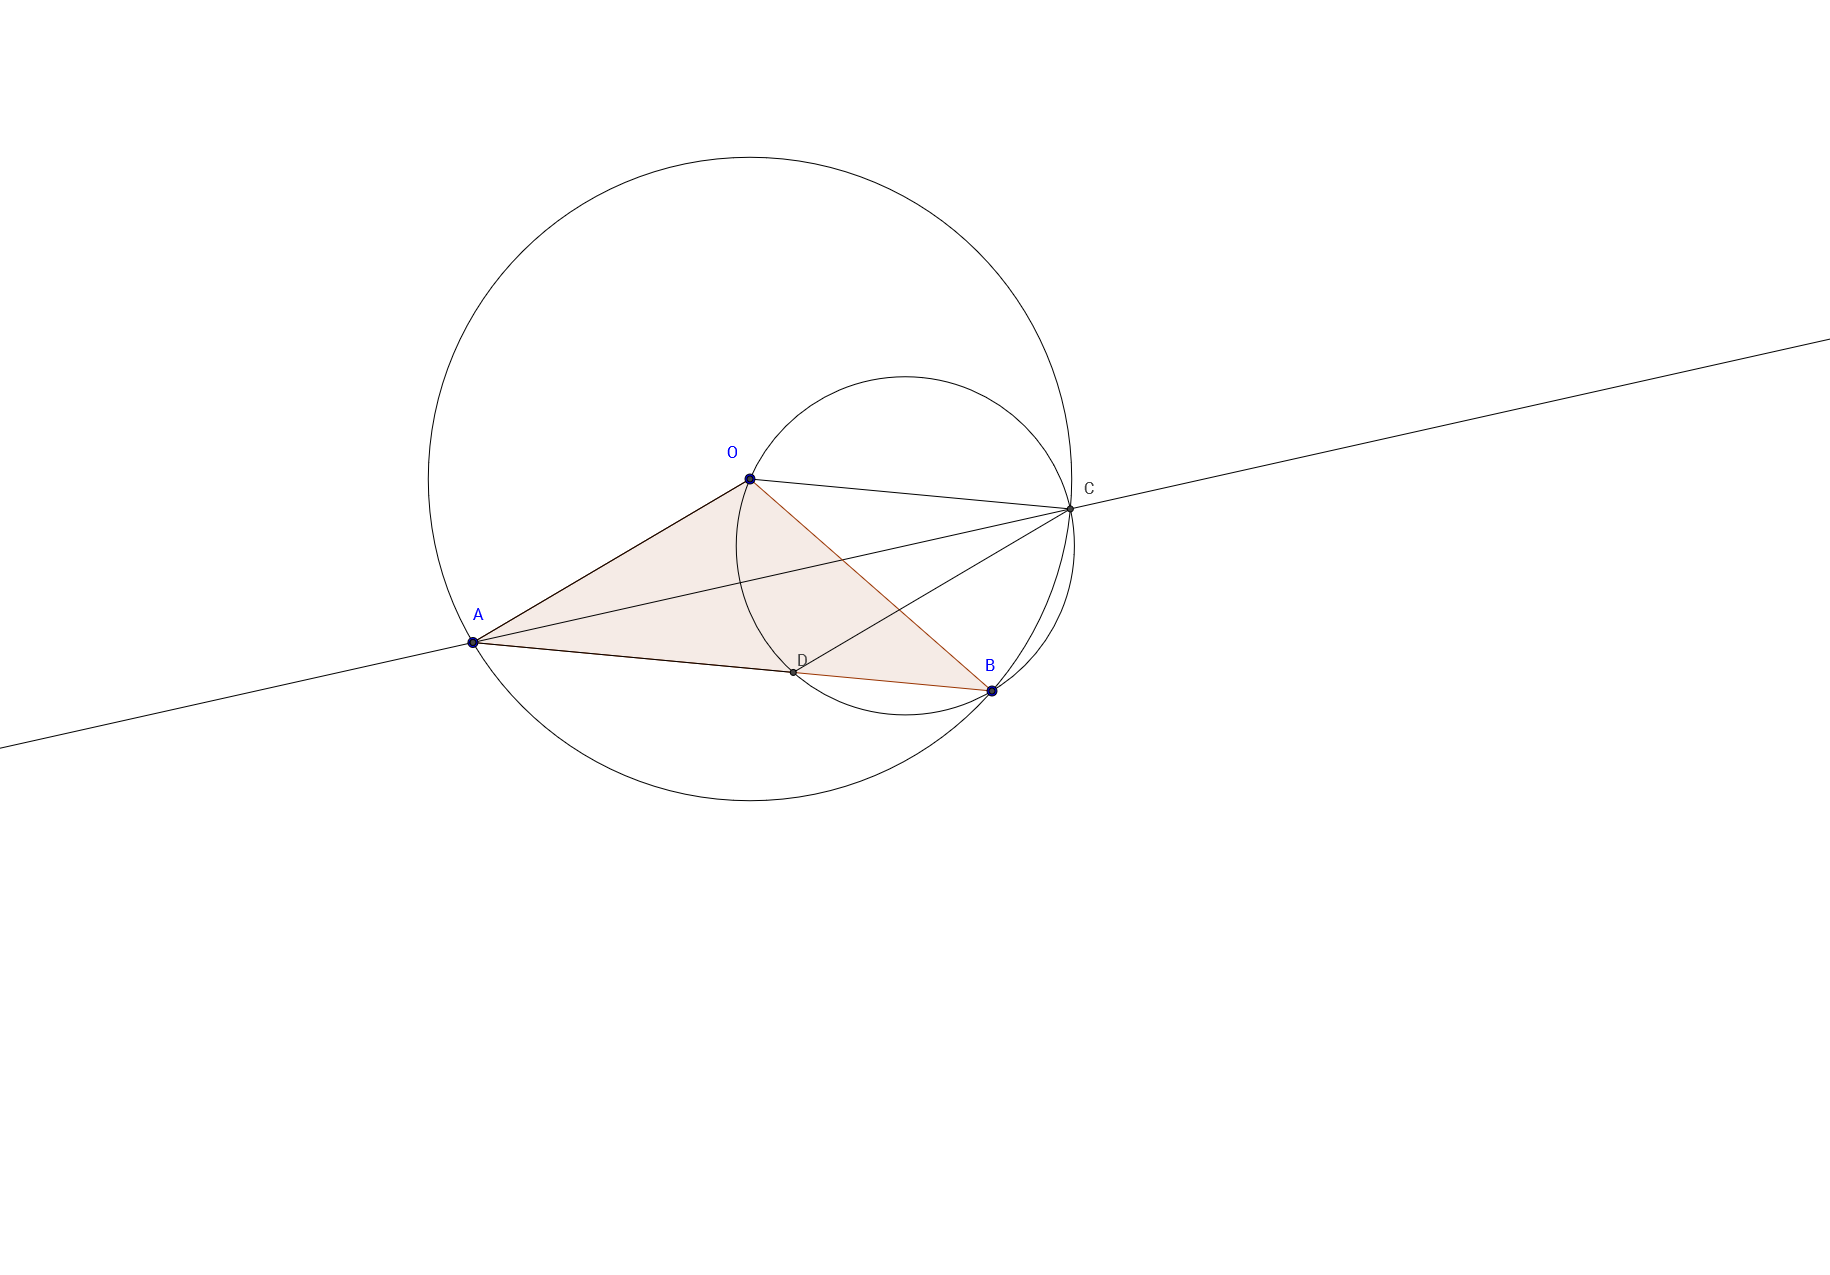
\includegraphics[width=\textwidth]{finalrunde_1_2017.png}

\textbf{Marking Scheme:}
\begin{itemize}
    \item +1 $\angle OCA = \angle OAC$ und $\angle OBA = 2\angle OAC$.
    \item +1 $\angle ABO = \angle DCO$.
    \item +2 Finde die ähnliche Dreiecken.
    \item +3 Fertig.
\end{itemize}

\newpage

%2
\item
Finde alle Funktionen $f\colon\R \to\R$, sodass für alle $x,y \in \R$ gilt:
\[
	f(x+yf(x)) = f(xf(y)) - x + f(y+f(x)).
\]

\textbf{Lösung:} Wir setzen $x=y=0$ ein, um $f(f(0)) = 0$ zu erhalten. Mit $x=y=1$ wird die Gleichung zu $f(f(1)) = 1$. Mit diesen beiden Identitäten und einsetzen von $x=1$ und $y=0$ erhalten wir $f(1) = 0$. Dann gilt auch $1 = f(f(1)) = f(0)$. Durch Einsetzen von $y=0$ wird die Originalgleichung zu $f(f(x)) = x$. Setzen wir nun $x=1$ und benutzen die gefundenen Identitäten, erhalten wir schliesslich für alle $y \in \mathbb{R}$ die Lösung $f(y) = 1-y$. Einsetzen zeigt, dass dies wirklich eine Lösung ist.

\textbf{Marking Scheme:}
\begin{itemize}
	\item +1 $f(0) = 1$.
	\item +1 $f(1) = 0$.
	\item +1 $f(f(x)) = x$.
	\item +1 $f(f(x)) = 1-f(x)$.
	\item +1 $f$ ist injektiv (bei $1$).
	\item -1 Lösung nicht überprüfen.
\end{itemize}
Bei unvollständige Lösungen sind maximal $4$ Punkte zu erreichen.


\newpage

%3
\item
Das Hauptgebäude der ETH Zürich ist ein in Einheitsquadrate unterteiltes Rechteck. Jede Seite eines Quadrates ist eine Wand, wobei gewisse Wände Türen haben. Die Aussenwand des Hauptgebäudes hat keine Türen. Eine Anzahl von Teilnehmern der SMO hat sich im Hauptgebäude verirrt. Sie können sich nur durch Türen von einem Quadrat zum anderen bewegen. Wir nehmen an, dass zwischen je zwei Quadraten des Hauptgebäudes ein begehbarer Weg existiert.

Cyril möchte erreichen, dass sich die Teilnehmer wieder finden, indem er alle auf dasselbe Quadrat führt. Dazu kann er ihnen per Walkie-Talkie folgende Anweisungen geben: Nord, Ost, Süd oder West. Nach jeder Anweisung versucht jeder Teilnehmer gleichzeitig, ein Quadrat in diese Richtung zu gehen. Falls in der entsprechenden Wand keine Türe ist, bleibt er stehen.

Zeige, dass Cyril sein Ziel nach endlich vielen Anweisungen erreichen kann, egal auf welchen Quadraten sich die Teilnehmer am Anfang befinden.

\textbf{Lösung:} Sobald zwei Teilnehmer nach einer Anweisung auf dem selben Quadrat sind, werden sie danach immer auf dem selben Quadrat sein, da sie immer in die gleiche Richtung gehen. Somit reduzieren wir das Problem auf dasselbe Problem mit einem Teilnehmer weniger. Dadurch genügt es zu zeigen, dass wir zwei verschiedene Teilnehmer auf das gleiche Quadrat lotsen können. Denn dann können wir per Induktion eine beliebige Anzahl Teilnehmer auf dasselbe Quadrat lotsen. Betrachte nun zwei Teilnehmer $A$ und $B$, die auf verschiedenen Feldern sind. Sei $d$ die minimale Anzahl von Anweisungen, die man benötigt, um $A$ auf das Feld, wo $B$ zu diesem Zeitpunkt steht, zu lotsen.
Nun gibt man eine Anweisungsfolge, mit welcher $A$ auf das Feld von $B$ gelangt und $d$ lang ist. Falls $B$ sich mindestens einmal nicht bewegt, können wir nun eine Anweisungsfolge finden, welche maximal $d-1$ Anweisungen enthält und $A$ auf das  Quadrat lotst, wo sich $B$ zu diesem Zeitpunkt befindet. Falls $B$ nie stehen blieb, können wir die selbe Anweisungsfolge geben, ohne das $A$ einmal stehen bleibt. Nun machen wir das so oft, bis $B$ bei einer Anweisung stehen bleibt. Da  $A$ am Anfang nicht auf dem gleichen Feld wie $B$ ist, ist der Vektor $\vec{AB}$ verschieden von $0$. $A$ und $B$ verschieben sich jede Anweisungsfolge um diesen Vektor, falls $B$ nie stehen bleibt. Da das Hauptgebäude in alle Richtungen beschränkt ist, kann es nicht passieren, muss $B$ innert endlich vielen Anweisungsfolgen einmal stehen bleiben. Somit wird $d$ auch hier nach endlich vielen Anweisungen um eins kleiner geworden. Nun machen wir dasselbe mit der neuen kürzesten Anweisungsfolge. Da $d$ natürlich ist, und sie in endlichen vielen Anweiungen strikt kleiner wird, wird $d$ irgendwann $0$. Somit sind wir fertig.
$\\$
Alternativ kann man zuerst $A$ in eine Ecke lotsen. O.B.d.A. ist dies die Ecke im Nordosten. Nun gibt man die kürzeste Anweisungsfolge, welche den anderen $B$ in die selbe Ecke schickt. Da $B$ nicht schon in der Ecke ist, ist er westlicher oder südlicher als $A$. Somit kommt Ost öfters als West oder Nord öfters als Süd vor. Da $A$ nach der Anweisungsfolge nicht nördlicher oder östlicher als vorher sein kann, muss $A$ mindestens einmal stehen bleiben. Die restliche Argument funktioniert wie vorhin.

\textbf{Marking Scheme:}
\begin{itemize}
	\item +1 Schicke $A$ zu derzeitige Position von $B$, ohne dass $A$ stehen bleibt.
	\item +2 Wird $B$ geblockt, dann wird der Weg kürzer, sonst benutzen wir denselben Weg.
	\item +2 Begründe, dass $B$ irgendwann geblockt werden soll.
	\item +2 Fertig.
\end{itemize}

\newpage

%4
\item Sei $n$ eine natürliche Zahl und $p,q$ Primzahlen, sodass folgende Aussagen gelten:
\begin{align*}
pq &\div n^p + 2,\\
n + 2 &\div n^p + q^p.
\end{align*}
Zeige, dass es eine natürliche Zahl $m$ gibt, sodass $q \div 4^m n +2$ gilt.

\textbf{Lösung:}
Es gilt $p\div n^p+2$ also $n^p\equiv -2 \mod{p}$. Da dank Fermats kleinem Satz gilt $n^p\equiv m\mod{p}$ ist also $n\equiv-2\mod{p}$.Wir können somit $n=kp-2$ schreiben. Setzen wir dies in $n+2\div n^p+q^p$ ein bekommen wir 
\[
pk\div n^p+q^p,
\]
also 
\[
n^p\equiv -q^p\mod{p}.
\] 
Da $n^p\equiv -2\mod{p}$ und wiederum $q^p\equiv q\mod{p}$ gilt $q\equiv 2\mod{p}$. Wir schreiben nun $q=lp+2$. Wenn $q=2$ gilt, ist die Aussage $q\div n\cdot 4^m+2$ für jedes $m\geq 1$ wahr. Wenn $p=2$ ist, dann ist $q$ gerade und da beides Primzahlen sind, ist also $q=2$, die Aussage also bewiesen. Für den Rest der Aufgabe können wir annehmen, dass $p, q$ ungerade Primzahlen sind nun gilt $ggt{n, q}=1$ (da $q\div n^p+2$). Da $q=lp+2$ muss $l=2k+1$ ungerade sein. Wir betrachten nun $n^{q-1}$ modulo $q$. Da $q$ prim ist, gilt $n^{q-1}\equiv 1\mod{q}$. Wir können $q-1$ schreiben als $lp+1$, also $n^{q-1}\equiv n\cdot (n^{p})^l \equiv n\cdot (-2)^{2k+1}\equiv (-2)n4^k\equiv 1\mod{p}$. Multiplizieren wir die Gleichung mit $(-2)$, erhalten wir $n4^{k+1}\equiv-2\mod{p}$ also $q\div n4^{k+1}+2$, was genau die Bedingung ist, die wir zeigen wollten. 
	
\textbf{Marking Scheme:}
\begin{itemize}
	\item +2 $p\div q-2$.
	\item +1 Idee haben, $m$ zu finden sodass $4^m \equiv n^{p-1}\mod q$.
	\item +4 Fertig.
	\item -1 Nicht sagen, dass $\frac{q-2}{p}$ ungerade ist.
	\item -1 Den Fall $q\div n$ vergessen.
\end{itemize}

\newpage

%5
\item Sei $ABC$ ein Dreieck mit $AC > AB$. Sei $P$ der Schnittpunkt von $BC$ und der Tangente durch $A$ am Umkreis des Dreiecks $ABC$. Sei $Q$ der Punkt auf der Geraden $AC$, sodass $AQ = AB$ gilt und $A$ zwischen $C$ und $Q$ liegt. Seien $X$ respektive $Y$ die Mittelpunkte von $BQ$ respektive $AP$. Sei $R$ der Punkt auf $AP$, sodass $AR=BP$ gilt und $R$ zwischen $A$ und $P$ liegt. Zeige, dass $BR = 2XY$ gilt.

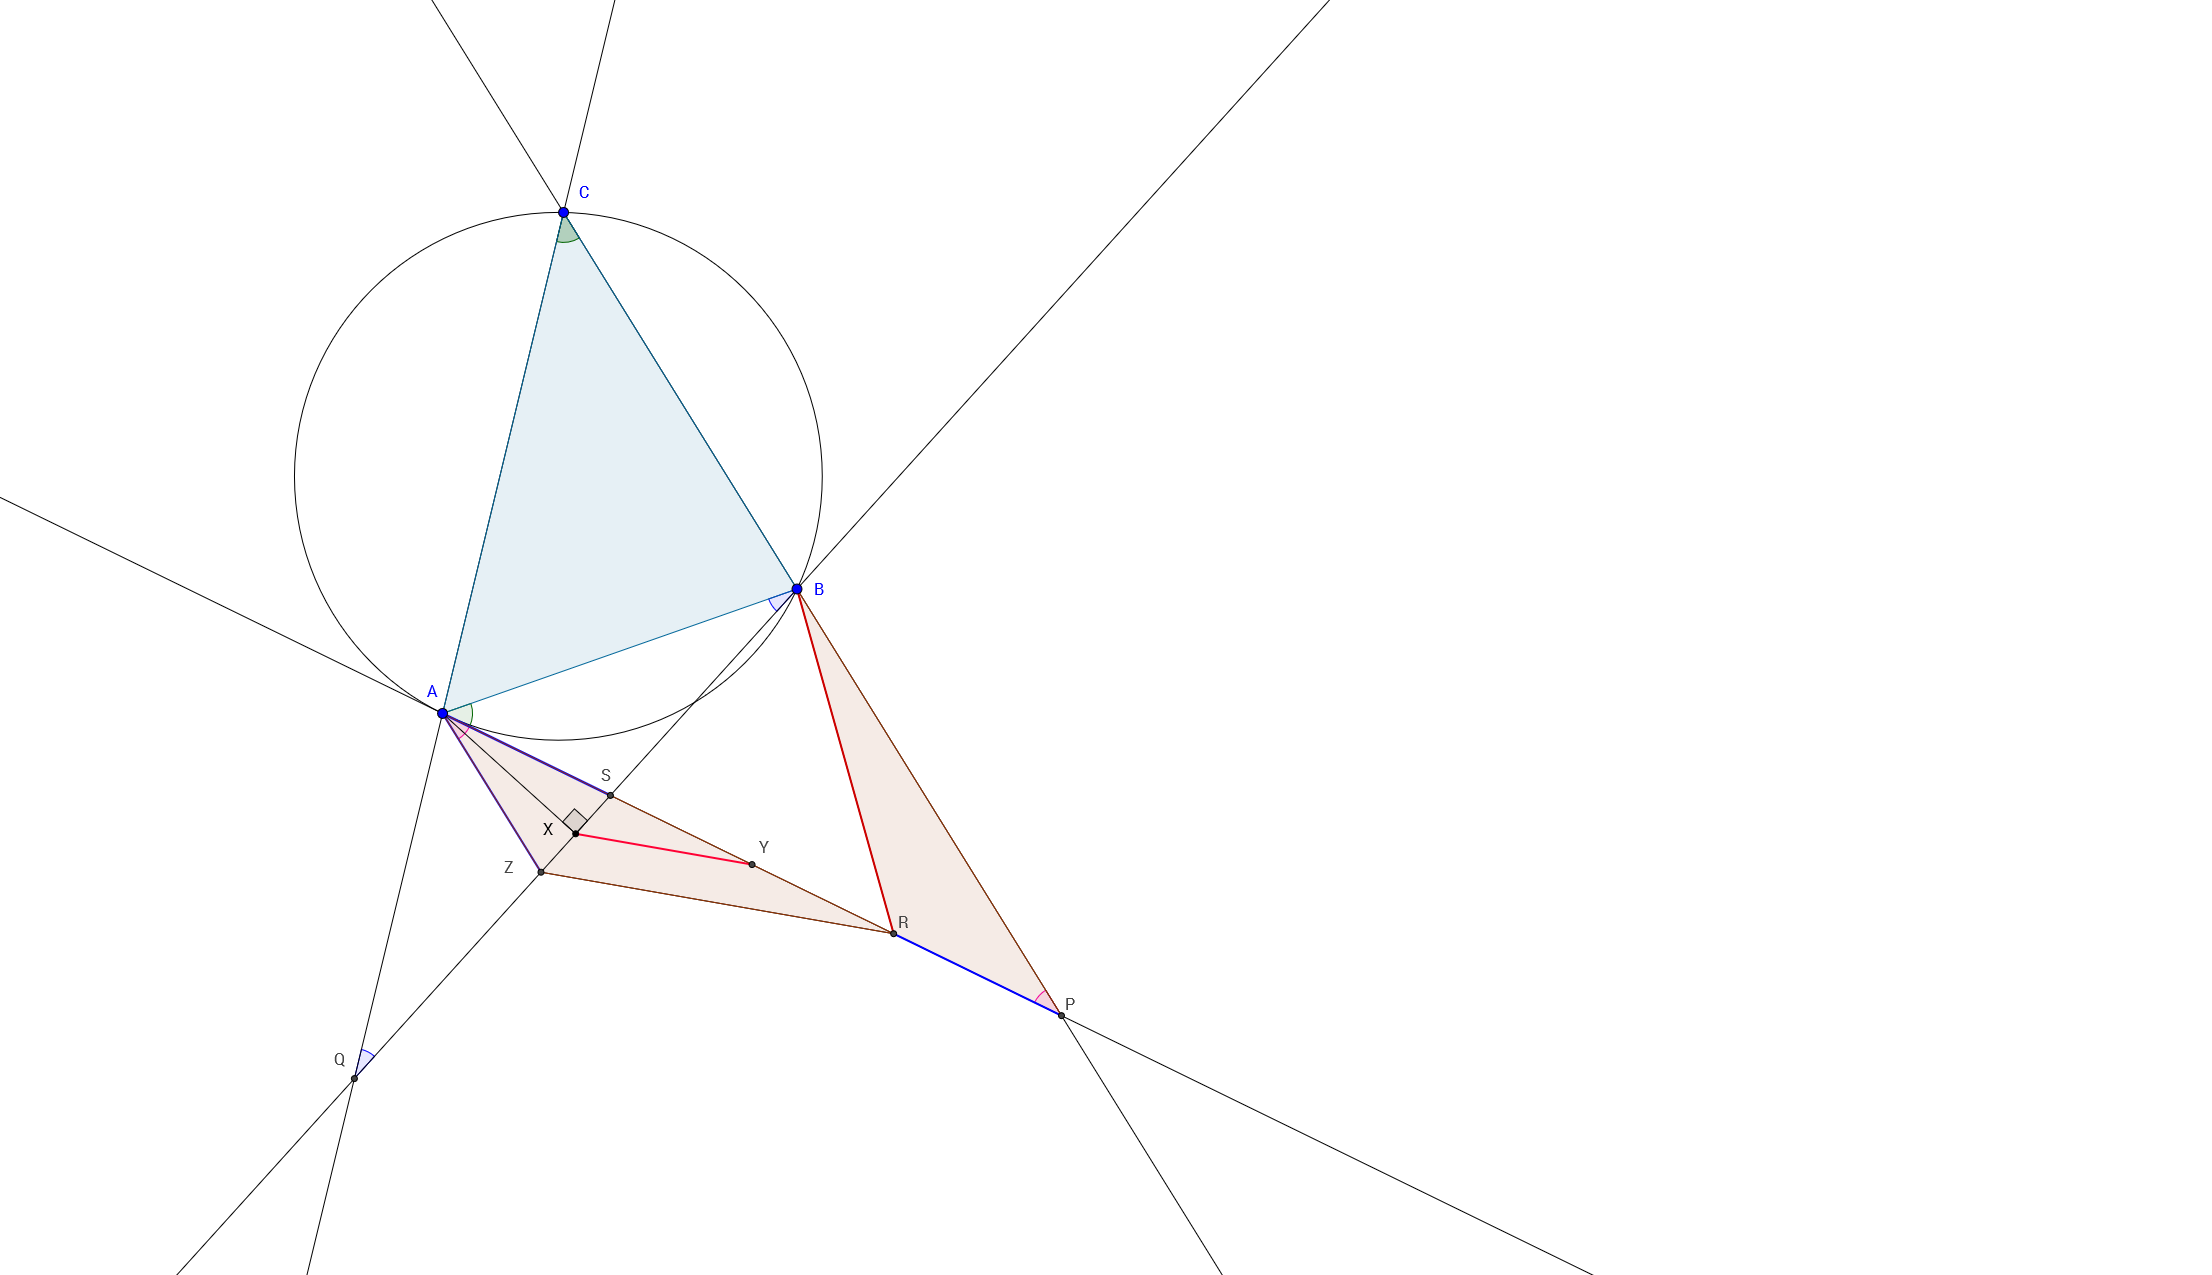
\includegraphics[width=\textwidth]{finalrunde_5_2017.png}

\textbf{Lösung:} Sei $S$ der Schnittpunkt von $AP$ und $BQ$. Wegen dem Tangentenwinkelsatz gilt $\angle SAB = \angle ACB = \angle QCB$ und nach Voraussetzung gilt $\angle ABS = \angle BQC$. Daraus folgt, dass die Dreiecke $ABS$ und $BQC$ ähnlich sind. Folglich sind die Nebenwinkel $ \angle PSB$ und $\angle SBP$ gleich gross und daraus folgt, dass $SP = BP = AR$ gilt, also auch $AS = AP - SP = AP - AR = RP$ und weil $Y$ der Mittelpunkt der Strecke ist auch $SY = YR$, Wir können nun also  $R$ als den Punkt betrachten, der entsteht, wenn man $Y$ von $S$ mit dem Faktor $2$ streckt. Mit dieser Motivation führen wir $Z$ auf der Strecke $BQ$ ein, so dass $SX = XZ$ gilt. Aus dem V-Strahlensatz folgt dann $2XY = ZR$ und es genügt zu zeigen, dass $ZR = AR$ gilt.
Da $ABQ$ gleichschenklig ist, steht $AX$ senkrecht auf $BQ$. Daher ist $Z$ ebenfalls die Spiegelung von $S$ an $AX$ und es gilt $AZ = AS = RP$ und $ \angle SZA = \angle ASZ = \angle PSB = \angle SBP$, also auch $\angle ZAR = \angle ZAS = \angle BPS = \angle BPR$. Daraus und aus $BP$ = $AR$ folgt mit der Umkehrung des V-Strahlensatzes, dass $AZR$ und $PRB$ kongruent sind, also auch $ZR = RB$ gilt.

\textbf{Marking Scheme:} 
\begin{itemize}
	\item +1 $AS = RP$.
	\item +2 $Z$ (oder ein anderer sinnvoller Punkt) einführen.
	\item +1 andere Eigenschaft von $Z$ beweisen.
	\item +1 $ZR = 2XY$ und Kongruenz von Dreiecken.
	\item +2 Fertig.
\end{itemize}

\newpage

%6
\item Au camp SMO, il y a au moins quatre Romands. Deux Romands sont soit mutuellement amis, soit mutuellement ennemis. Dans chaque groupe de quatre Romands, au moins un des Romands est ami avec les trois autres. Existe-t-il toujours un Romand qui est ami avec tous les autres?

\textbf{Solution:} On numérote les personnes $P_1, P_2, \ldots, P_n$. Considérons la première personne $P_1$. Si $P_1$ est ami avec tout le monde, l'exercice est terminé. Autrement on peut supposer sans perte de généralité que $P_1$ et $P_2$ ne sont pas amis. Alors, dans le groupe $P_1, P_2, P_3, P_4$ une des personnes est amie avec les trois autres, et par supposition ce n'est ni $P_1$, ni $P_2$. On peut donc supposer que $P_3$ est ami avec les trois autres personnes du groupe. Nous allons montrer maintenant que $P_3$ est alors ami avec tout le monde.
	
Nous savons déjà que $P_3$ est ami avec $P_1, P_2$ et $P_4$. Considérons n'importe quelle autre personne $P_k$. Alors dans le groupe $P_1, P_2, P_3, P_k$ une des personnes est amie avec tout le monde, et nous avons déjà vu que cette personne ne peut être ni $P_1$, ni $P_2$. Ainsi cette personne est soit $P_3$, soit $P_k$, et dans les deux cas $P_3$ et $P_k$ sont amis donc, comme $P_k$ était choisi arbitrairement, $P_3$ est bien ami avec tout le monde.

\textbf{Marking Scheme:}
\begin{itemize}
	\item +2 Il n'existe pas deux paires disjointes d'ennemis.
	\item +2 $L_i$ et $L_j$ sont amis pour toutes les paires avec $3\leq i < j \leq n$.
	\item +3 Terminer.
\end{itemize}

\newpage

%7
\item Sei $n$ eine natürliche Zahl, sodass es genau $2017$ verschiedene Paare natürlicher Zahlen $(a,b)$ gibt, welche die Gleichung
\[
 \frac{1}{a} + \frac{1}{b} = \frac{1}{n}
\]
erfüllen. Zeige, dass $n$ eine Quadratzahl ist.

\textit{Bemerkung: $(7,4) \neq (4,7)$}

\textbf{Lösung:}
Bemerke, dass $a$ und $b$ beide grösser als $n$ sind. Wir multiplizieren die Gleichung mit $nab$ und bekommen $bn+an=ab$. Nach Addition von $n^2$ subtrahieren wir $bn+an$ und können faktorisieren: $(a-n)(b-n)=n^2$. Da $a$ und $b$ grösser als $n$ sind, bekommen wir eine Bijektion von geordneten Paaren $(s,n^2/s)$, wobei $s$ ein Teiler von $n^2$ ist, und geordneten Paaren $((a-n),(b-n))$ und somit ebenfalls eine Bijektion von $(s,n^2/s)$ auf geordnete Lösungspaare $(a,b)$. Da es genau 2017 geordnete Lösungspaare gibt, hat folglich $n^2$ genau 2017 verschiedene Teiler. 2017 ist prim, also gilt $n^2 = p^{2016}$ für ein Primzahl $p$, und dann gilt $n = p^{1008}$ ist ein Quadratzahl, wie gewünscht.

\textbf{Marking Scheme:}
\begin{itemize}
	\item +2 $(a-n)(b-n) = n^2$.
	\item +2 Bijektion zwischen Lösungsmenge und Teiler von $n^2$.
	\item +3 Fertig.
	\item -1 Negative Teiler vergessen.
\end{itemize}
Eine andere sinnvolle Bijektion ist $4$ Punkte wert.

\newpage

%8
\item Sei $ABC$ ein gleichschenkliges Dreieck mit Scheitelpunkt $A$ und $AB > BC$. Sei $k$ der Kreis mit Zentrum $A$ durch $B$ und $C$. Sei $H$ der zweite Schnittpunkt von $k$ mit der Höhe des Dreiecks $ABC$ durch $B$. Weiter sei $G$ der zweite Schnittpunkt von $k$ mit der Schwerlinie durch $B$ im Dreieck $ABC$. Sei $X$ der Schnittpunkt der Geraden $AC$ und $GH$. Zeige, dass $C$ der Mittelpunkt der Strecke $AX$ ist.

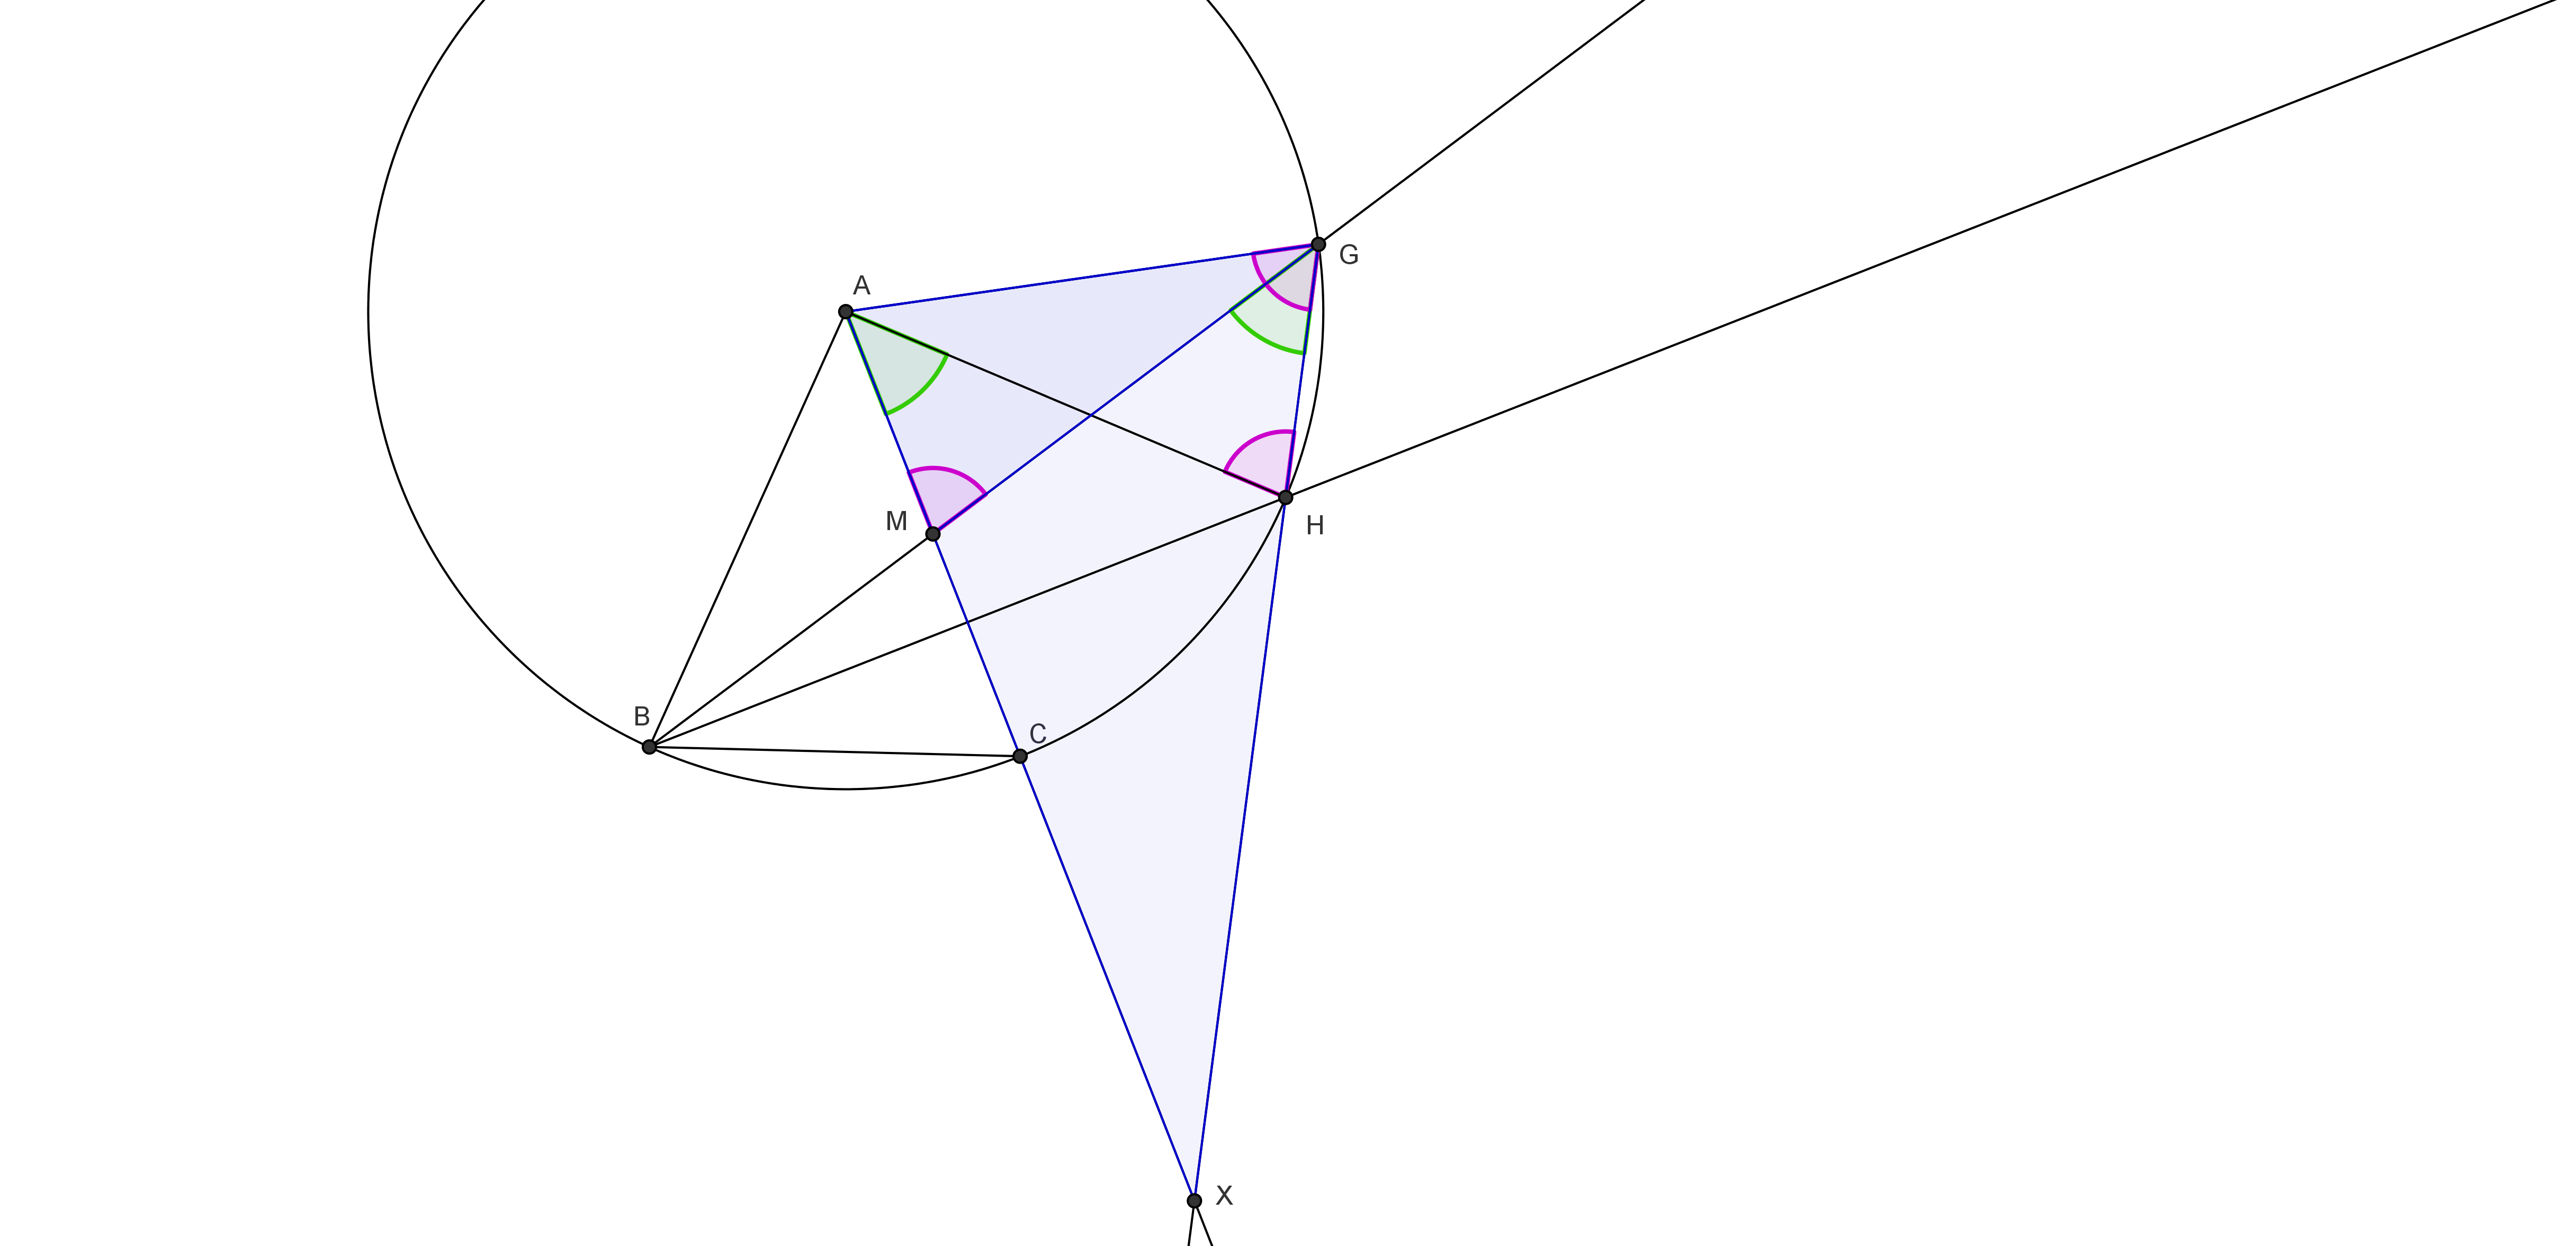
\includegraphics[width=\textwidth]{finalrunde_8_2017.png}

\textbf{Lösung:}
Sei $M$ der Mittelpunkt der Strecke $AC$. Mit dem Zentriwinkelsatz erhält man $\angle BGH=\frac{1}{2}\angle BAH$. Da das Dreieck $ABH$ gleichschenklig ist und die Strecke $BH$ senkrecht zu der Stecke $AC$ steht, ist $AC$ die Winkelhalbierende von Winkel $BAH$. Daher gilt:
\[
\angle BGH = \angle CAH = \angle MAH
\]
Mit dem Peripheriewinkelsatz erhält man das Sehnenviereck $MAGH$. Mit diesem Sehnenviereck erhält man $\angle AMG=\angle AHG$. Da Dreieck $AHG$ gleichschenklig ist gilt
\[
\angle AGH=\angle AHG=\angle AMG.
\]
Daher ist Dreieck $AMG$ ähnlich zu Dreieck $AGX$. Da $M$ der Mittelpunkt von $AC$ ist, erhält man mit den Seitenverhältnissen:
\[
\frac{AG}{AX}=\frac{AM}{AG}=\frac{AM}{AC}=\frac{1}{2}
\]
Wir berechnen:
\[
AC = AG = \frac{1}{2} AX
\]
Somit ist $C$ der Mittelpunkt der Strecke $AX$.

\textbf{Marking Scheme:}
\begin{itemize}
	\item +2 Zwei sinnvolle Winkel.
	\item +2 Zwei sinnvolle ähnliche Dreiecke.
	\item 5 Sinnvolle Verhältnisse zwischen Seitenlängen.
	\item 7 Fertig.
\end{itemize}

\newpage

%9
\item Betrachte ein konvexes $15$-Eck mit Umfang $21$. Zeige, dass man davon drei paarweise verschiedene Eckpunkte auswählen kann, die ein Dreieck mit Fläche kleiner als $1$ bilden.

\textbf{Lösung:} Nenne die 15 Seiten $a_1,\ldots, a_{15}$ und definiere $a_{16} = a_1$. Betrachte die Summen $b_i=a_i+a_{i+1}$ für $i=1,\ldots,15$. Dann gilt $b_1+\ldots+b_{15}=2(a_1+\ldots+a_{15})=42$. Mit Schubfachprinzip folgt, dass es ein $b_i\leq \frac{42}{15}=\frac{14}{5}$ gibt. Das Dreieck, das die beiden Seitenlängen $a_i$ und $a_{i+1}=b_i-a_i$ hat, kann folglich höchstens die Fläche $\frac{1}{2}a_i(b_i-a_i)$ aufspannen, also höchstens $\frac{1}{2}a_i(\frac{14}{5}-a_i)$. Wir wollen also zeigen, dass $\frac{1}{2}a_i(\frac{14}{5}-a_i) < 1$ gilt. Dies können wir umschreiben als $\frac{14}{5}a_i\leq a_i^2+2$.  Mit AM-GM folgt $a_i^2+2\geq 2\sqrt{2}a_i$ und $\sqrt{2}>\frac{7}{5}$, also sind wir fertig.

\textbf{Marking Scheme:}
\begin{itemize}
	\item +2 Zwei nebeneinanderliegenden Seiten zusammen $\leq 14/5$.
	\item +1 Fläche des Dreiecks mit Seitenlängen $a_1, a_{i+1} \leq a_ia_{i+1}/2$.
	\item +1 Abschätzung mit AM-GM oder Ähnliches.
	\item +3 Fertig.
\end{itemize}

\newpage

%10
\item Soient $x,y,z$ des nombres réels positifs ou nuls avec $xy + yz + zx = 1$. Montrer que
\[
\frac{4}{x+y+z} \leq (x + y)(\sqrt{3}z + 1).
\]

\textbf{Première solution:}
On réécrit l'équation sous la forme
\[
	4 \leq (x+y+z)(x+y)(\sqrt{3}z+1) = (x^2 + 2xy + x^2 + xz + yz)(\sqrt{3}z +1) = \sqrt{3}z(x^2 + 2xy + y^2 + xz + yz) + x^2 + xy + y^2 + 1.
\]

On peut encore transformer pour obtenir $3 \leq \sqrt{3}z(x^2 + 2xy + y^2 + xz + yz) + x^2 + xy + y^2$ et puisque par AM-GM $x^2 + xy + y^2 \geq 3xy$, il suffit de prouver
\[
	1 \leq \frac{1}{\sqrt{3}}(x^2z + xyz + y^2 + xz^2 + yz^2) + xy \Leftrightarrow yz + xz \leq \frac{1}{\sqrt{3}}(x^2z + xyz + y^2 + xz^2 + yz^2).
\]

Le terme de droite peut se factoriser comme
\[
	\frac{1}{\sqrt{3}}(x^2z + xyz + y^2 + xz^2 + yz^2) = \frac{1}{\sqrt{3}}(xz + yz)(x + y + z),
\]
donc si on prouve que $x + y + z \geq \sqrt{3}$ l'inéquation est alors démontrée puisqu'on a clairement $xz + yz \geq 0$. On a en fait $(x + y + z)^2 = x^2 + y^2 + z^2 + 2(xy + yz + zx) \geq 3(xy + yz + zx) = 3$, ce qui conclut la preuve.

\textbf{Deuxième solution:}
On commence par réécrire l'inéquation sous la forme
\[
	4 \leq (x+y+z)(x+y)(\sqrt{3}z + 1).
\]
On remarque que l'inéquation et la condition sont toutes les deux symétriques en $x$ et $y$ (c'est-à-dire: rien ne change si on échange $x$ et $y$), donc on suppose que le minimum devrait être atteint lorsque $x = y$. Prenons trois variables $x, y, z$ avec $xy +yz + zx = 1$. Nous allons regarder ce qu'il se passe avec le côté droit lorsqu'on les remplace par 
\[
	x' = \frac{x+y}{2}, y' = \frac{x+y}{2}, z'
\]
avec $x'y' + y'z' + z'x' = 1$. La condition sur les variables est équivalente à
\[
	z= \frac{1-xy}{x+y} \qquad z' = \frac{1-x'y'}{x'+y'} = \frac{1-\left(\frac{x+y}{2}\right)^2}{x+y}.
\]

Si $x + y \leq 2$ on a donc que $x', y', z'$ sont tous positifs et on peut alors regarder l'inéquation avec ces nouvelles variables. Autrement, on a $x+y > 2$, $x + y + z \geq x + y >2$ et $\sqrt{3}z + 1 \geq 1$. L'inéquation est ainsi trivialement vérifiée et on exclut donc ce cas pour la suite.

Par AM-GM on sait que $\left(\frac{x+y}{2}\right)^2 \geq xy$, donc $z' \leq z$. Ainsi, puisque l'on a $x+y = x' + y'$ et $z \geq z'$ on voit que le côté droit diminue avec ces nouvelles variables, donc il suffit de prouver l'inéquation dans le cas $x = y \leq 1$. La condition devient alors $x^2 + 2xz = 1$ et l'inéquation s'écrit
\[
	4 \leq (2x + z)2x(\sqrt{3}z + 1) = (4x^2 + 2xz)(\sqrt{3}z + 1) = (3x^2 + 1)(\sqrt{3}z + 1).
\]

En développant le terme de droite, on obtient $3\leq 3\sqrt{3}x^2z + \sqrt{3}z + 3x^2$, qui est elle-même équivalente à $3\cdot 2xz \leq 3\sqrt{3}x^2z + \sqrt{3}z$; cette dernière inéquation se laisse facilement prouver par votre inéquation favorite.

\textbf{Troisième solution:}
Pour commencer, on identifie les cas d'égalité. Il est important de remarquer à ce stade qu'il existe au moins deux cas d'égalité:
\[
(x,y,z)\in\left\{(1,1,0),\left(\frac{1}{\sqrt{3}},\frac{1}{\sqrt{3}},\frac{1}{\sqrt{3}}\right)\right\}.
\]
La symétrie en $x$ et $y$, suggère la substitution suivante : $s:=x+y$ et $t:=xy$. De la condition, on obtient $z=\frac{1-t}{s}$. On peut donc réécrire l'inéquation de la manière suivante :
\[
4s\leq (s^2+1-t)(s+\sqrt{3}(1-t)).
\]
Notons à présent que AM-GM fournit la relation $s^2\geq 4t$. De plus, utilisant la condition initiale, $1-t\geq 0$. En gardant en mémoire les cas d'égalités, à savoir $(s,t)=(2,1)$ et $(s,t)=(2/\sqrt{3},1/3)$, on peut aboutir à la factorisation suivante (la factorisation doit mettre en évidence les cas d'égalités !):
\[
(s^2+1-t)(s+\sqrt{3}(1-t))-4s=s(s^2-4t)+\frac{\sqrt{3}}{4}(1-t)\left((s^2-4t)+(\sqrt{3}s-2)^2\right).
\]
Le coté droit étant positif, on a terminé.

\textbf{Première solution:}
\begin{itemize}
	\item +5 Réduire l'inéquation à $x + y + z \geq \sqrt{3}$.
	\item +2 Terminer.
\end{itemize}
\textbf{Deuxième solution:}
\begin{itemize}
	\item +3 Réduire au cas $x = y$.
	\item +4 Terminer.
	\item -2 Oublier le cas $x + y > 2$.
\end{itemize}
\textbf{Troisième solution:}
\begin{itemize}
	\item +1 Introduire $s$ et $t$ et prouver $s^2 \geq 4t$.
	\item +6 Terminer.
\end{itemize}


\end{enumerate}

\bigskip

\vspace{1cm}

\end{document}
